\chapter{Output Stage and Power Amplifiers}

Output stage and power amplifiers must be capable of processing some of the highest voltages and currents of a circuit design.
A common use for output stage amplifiers is to amplify the power of a voltage signal representing a sound. In this application, pre-amplifiers operate on very small input signals (such as from a microphone), summing amplifiers mix the input signals, and the output stage amplifier processes the mixed input signals and drive a speaker.

To reduce power consumption and the circuit's supply voltage without lowering the maximum output voltage swing, these amplifiers usually require an output voltage swing that is nearly rail-to-rail, is rail-to-rail, or in some cases is greater than rail-to-rail.
This requirement, along with the relatively high voltages and currents processed by these circuits, often results in loss of linearity as the output stage transistors operate on signals that are too large for typical small signal assumptions to remain valid.
Many output stage and power amplifiers must thus also be designed to minimize these nonlinearities caused by large signals since nonlinearities cause harmonic distortions and other undesirable behaviors.
In the case of audio signals, nonlinearities produce audible and very undesirable distortions which significantly reduce the quality of the audio signal.

Another consideration for output stage and power amplifiers is that output stage/power transistors must be designed differently from the transistors that process smaller signals (such as the transistors in pre-amplifiers) in order to ensure that the signals processed by the output stage or power amplifier remain in all the transistors' \ac{soa}.
Unfortunately, increasing the \ac{soa} for output stage/power transistors reduces their performance in other areas -- such as the unity gain frequency ($f_{T}$) or, in the case of bipolar transistors, current gain ($\beta$).

With all these design challenges, output stage and power amplifiers are divided into classes based on the percent of time the output stage/power transistors are conducting (the amplifier's power efficiency).
These classifications include class A, B, AB, C, D, E, F, G, and H amplifiers.
The transistors in a class A amplifier conduct for the entire cycle of a sine wave input signal and so are the least power efficient.
A simple example of a class A amplifier is the common emitter.
Transistors in class B amplifiers conduct for half the cycle of a sine wave, and transistors in a class AB amplifier are biased at a low quiescent current and conduct for slightly more than half a cycle. \autocite[574-575]{microelectronics-neaman}
%TODO: Discuss C, D, E, F, G, and H amplifiers from other sources

Although output stage amplifiers and power amplifiers often share similar designs, there is an important distinction:
power amplifiers are designed to maximize the power $P_{L} = V_{L}I_{L}$ delivered to a load while output stage amplifiers are designed to maximize voltage swing and minimize output impedance.
The applications for each type of amplifier differs slightly, too;
power amplifiers are used to drive speakers or an antenna -- to transmit \iac{rf} signal, for example -- while an output stage amplifier is used for applications such as the output stage of op amps.

\section{Class A Amplifiers}

\subsection{Inductively coupled class A amplifier}
\begin{center}
		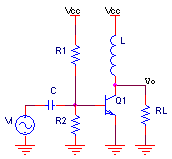
\includegraphics{schematics/inductivecommonemitter.png}
\end{center}
This is a common emitter circuit with an inductor in place of the collector resistor. The inductor should be chosen such that

\begin{equation}
\omega L \gg R_{L}
\end{equation}

for all signal frequencies $\omega$.
If this is true then the inductor is a short circuit to \DC and all frequencies below those of interest, and an open circuit to the frequencies of interest.
Since there is no emitter resistor

\begin{equation}
I_{C} = \frac{V_{CE}}{R_{L}} = \frac{V_{CC}}{R_{L}}
\end{equation}

The latter equation holds true since $L$ is a short at \DC.
$I_{C}$ is the maximum signal current because

\begin{equation}
i_{c} = \frac{-v_{ce}}{R_{L}} \leq \frac{-V_{CC}}{R_{L}}
\end{equation}

since the impedance of $L$ increases with frequency (and thus $v_{CE}$ is maximized at \DC).
The maximum possible average signal power delivered to $R_{L}$ is

\begin{equation}
\overline{P_{L}} = \frac{1}{2}I_{C}^{2}R_{L} = \frac{1}{2}\frac{V_{CC}^{2}}{R_{L}}
\end{equation}

Ignoring the power dissipated by the bias resistors $R_1$ and $R_2$, the average power dissipated by the amplifier is

\begin{equation}
\overline{P_{D}} = I_{C}V_{CC} = \frac{V_{CC}}{R_{L}}
\end{equation}

The (theoretical) maximum possible power conversion efficiency is thus \autocite[588-589]{microelectronics-neaman}

\textcolor{red}{
\begin{equation}
\eta = \frac{\overline{P_{L}}}{\overline{P_{D}}} = \frac{\frac{1}{2}\frac{V_{CC}^{2}}{R_{L}}}{\frac{V_{CC}^{2}}{R_{L}}} = \frac{1}{2}
\end{equation}
}

If the inductor is instead a resistor and the transistor biased so that $V_{CE} = \frac{V_{CC}}{2}$ (to maximize the possible signal swing in both positive and negative directions), then for a sinusoidal signal

\begin{equation}
i_{C} = I_{C} + i_{i}\sin{\omega t}
\end{equation}

and

\begin{equation}
v_{C} = \frac{V_{CC}}{2} - v_{i}\sin{\omega t}
\end{equation}

where $i_{i}$ and $v_{i}$ are the input current and voltage, respectively.
Thus, the maximum

\begin{equation}
i_{C(\text{max})} = I_{C}
\end{equation}

and

\begin{equation}
v_{C(\text{max})} = \frac{V_{CC}}{2}
\end{equation}

so

\begin{equation}
\overline{P_{L}} = \frac{1}{2}I_{C}\frac{V_{CC}}{2} = \frac{I_{C}V_{CC}}{4}
\end{equation}

As before

\begin{equation}
\overline{P_{D}} = I_{C}V_{CC}
\end{equation}

so the maximum possible power conversion efficiency is only \autocite[575-576]{microelectronics-neaman}

\textcolor{red}{
\begin{equation}
\eta = \frac{\overline{P_{L}}}{\overline{P_{D}}} = \frac{\frac{1}{4}I_{C}V_{CC}}{I_{C}V_{CC}} = \frac{1}{4}
\end{equation}
}

The inductively coupled class A amplifier is thus considerably more power efficient than a simple common emitter.

\subsection{Transformer-coupled class A amplifier}
\begin{center}
		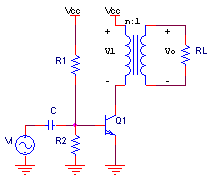
\includegraphics{schematics/transformercommonemitter.png}
\end{center}
The inductively coupled class A amplifier design depends in part on the load resistance $R_{L}$, so it may be difficult to acheive a power conversion efficiency near the theoretical maximum of \SI{50}{\percent}.
The load resistance seen by the amplifier can be optimized by using a transformer with a specific turns ratio.
For a turns ratio of $n:1$ the current $i_{L}$ through the load resistance $R_{L}$ is related to the collector current $i_{C}$ by

\begin{equation}
i_{L} = ni_{C}
\end{equation}

Similarly, the voltage $v_{O}$ across the load is related to the voltage from $V_{CC}$ to the voltage at the transistor's collector ($v_{1}$ in the schematic) by

\begin{equation}
v_{O} = nv_{1}
\end{equation}

By definition

\begin{equation}
R_{L} = \frac{v_{O}}{i_{L}}
\end{equation}

so the transformed load resistance (that is, the resistance seen by the transistor) is

\begin{equation}
R_{L}' = n^{2}R_{L}
\end{equation}

By choosing an appropriate $R_{L}'$ using the transformer's turns ratio the same analysis can be applied to the transformer-coupled amplifier as the inductively coupled amplifier to achieve a (theoretical) maximum power conversion efficiency \autocite[589-590]{microelectronics-neaman}

\textcolor{red}{
\begin{equation}
\eta = \frac{1}{2}
\end{equation}
}

\subsection{Transformer-coupled emitter follower amplifier}
\begin{center}
		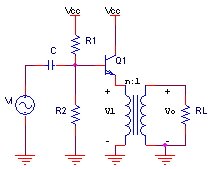
\includegraphics{schematics/transformeremitterfollower.png}
\end{center}
The transformer-coupled emitter follower does not provide a voltage gain like most amplifiers do, but its low output impedance makes it a useful final stage for many amplifiers.
As with the preceding circuit, the transformer alters the load resistance seen by the transistor to

\begin{equation}
R_{L}' = n^{2}R_{L}
\end{equation}

Since the emitter follower has a voltage gain

\textcolor{red}{
\begin{equation}
\frac{\vout}{\vin} \approx 1
\end{equation}
}

and the maximum output voltage is

\begin{equation}
v_{O} = \frac{v_{1}}{n} = \frac{V_{CC}}{n}
\end{equation}

(since the emitter voltage can go no higher than $V_{CC}$ and $v_{O} = \frac{v_{1}}{n}$) the average power delivered to the load is simply

\begin{equation}
\overline{P_{L}} = \frac{1}{2}\frac{V_{CC}^{2}/2}{n^{2}R_{L}}
\end{equation}

The average power dissipated is

\begin{equation}
\overline{P_{D}} = \frac{V_{CC}^{2}/2}{n^{2}R_{L}}
\end{equation}

so \autocite[591]{microelectronics-neaman}

\textcolor{red}{
\begin{equation}
\eta = \frac{\overline{P_{L}}}{\overline{P_{D}}} = \frac{1}{2}
\end{equation}
}

\section{Class B Amplifiers}

\subsection{Class B bipolar push-pull output stage}
\begin{center}
	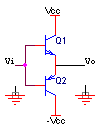
\includegraphics{schematics/classBoutput.PNG}
\end{center}
This class B amplifier is a \textit{complementary} output stage because it uses both \textit{npn} and \textit{pnp} transistors.
Class B output stages such as these are typically implemented in integrated circuits only since the two transistors must be well matched for optimal behavior.
Class A output stages dissipate significant power even when there is no input signal (since the single transistor in the class A output stage as always on), but class B output stages have very low power dissipation with no input signal because each of the two transistors is only on for about half the signal cycle and neither is on when there is no input signal.

There are three distinct regions of the transfer characteristic for this class B output stage.
The first is for $|v_{i}| < v_{BE(on)}$ (assuming the transistors are matched so that they have the same $v_{BE(on)}$).
In this case neither transistor is on so

\textcolor{red}{
\begin{equation}
v_{o} = 0\text{, }|v_{i}| < v_{BE(\text{on})}
\end{equation}
}

The second region is for $v_{BE(\text{on})} < |v_{i}| < V_{CC} + v_{BE(\text{on})} - v_{CE(\text{sat})}$ (where $v_{CE(\text{sat})}$ is the value of $v_{CE}$ above which the transistor enters the saturation region).
If \vin satisfies this condition and is positive then $Q_1$ is active and $Q_2$ is off;
if \vin is negative then $Q_2$ is active and $Q_1$ is off.
The active transistor acts as an emitter follower since its collector is at \AC ground and the output is taken from its emitter.
Thus,

\textcolor{red}{
\begin{equation}
\vout = \vin\text{, }v_{BE(\text{on})} < |\vin| < V_{CC} + v_{BE(\text{on})}-v_{CE(\text{sat})}
\end{equation}
}

in this region.
The third region is caused by the saturation of the active transistor. In this region the output does not change with the input:

\textcolor{red}{
\begin{equation}
v_{o} = V_{CC}-v_{CE1(\text{sat})}\text{, }v_{i} > V_{CC} + v_{BE1(on)} - v_{CE1(sat)}
\end{equation}
}

\textcolor{red}{
\begin{equation}
v_{o} = -V_{CC}+v_{CE2(\text{sat})}\text{, }v_{i} = -V_{CC}+v_{BE2}-v_{CE2(\text{sat})}
\end{equation}
}

The class B output stage unfortunately suffers from two types of distortion:
clipping and crossover distortion.
Clipping obviously occurs when the input signal has too high an amplitude for the output stage.
To avoid clipping, the supply voltage of the circuit must be increased or the input signal must have a low enough amplitude that the transistors do not enter the saturation region.
Unfortunately, the input signal cannot have too low an amplitude, either:
crossover distortion is the result of the fact that $\vout = 0$ for $|\vin| < v_{BE(on)}$.
With neither transistor active in this region (sometimes called the deadband), the output does not follow the input.
The only way to minimize the effect of crossover distortion is to ampilify the input signal sufficiently so that the deadband is only a small percentage of the input signal's amplitude, or to use a class AB output stage. \autocite[362-364]{analysis-design-analog-ics}

\subsection{Class B \textit{npn} bipolar output stage (GHLM p. 376)}
\begin{center}
	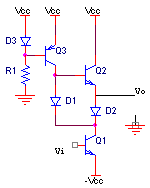
\includegraphics{schematics/npnClassBoutput.PNG}
\end{center}
This class B output stage, like the previous class AB output stage with Darlington pairs, takes into account the fact that \textit{pnp} transistors perform poorly compared to \textit{npn} transistors because \ac{ic} process technologies usually optimize the \textit{npn} transistors at the expense of the \textit{pnp} transistors.
This circuit is designed for higher power applications (several watts of output power or more) because the \textit{pnp} transistors are incapable of carrying higher currents.

%\subsection{Class B output stage with anti-cross-conduction (DC Analysis 4)}

\section{Class AB Amplifiers}

\subsection{Class AB bipolar output stage}
\begin{center}
	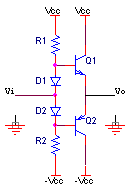
\includegraphics{schematics/classABoutput.PNG}
\end{center}
This class AB output stage eliminates the deadband (and the resulting crossover distortion) by adding two diodes and two resistors to the class B push-pull output stage.
The resistors bias the two diodes on, which forces a voltage drop across each diode (nearly all of the current through the resistors flows through the diodes since $I_{B}$ is a factor of $\beta_{F}$ smaller than the bias current).
The voltage drop across each diode creates a nonzero $V_{BE}$ so that $|\vin|$ no longer needs to overcome the transistors' $v_{BE(\text{on})}$ -- one of the transistors becomes active as soon as $\vin \neq 0$. \autocite[365]{analysis-design-analog-ics}
Other than correcting for the deadband region, the operation of the class AB output stage is nearly the same as that of the class B output stage:

\textcolor{red}{
\begin{equation}
\vout = \vin\text{, }|\vin| < V_{CC} + v_{BE(\text{on})}-v_{CE(\text{sat})}
\end{equation}
}

\textcolor{red}{
\begin{equation}
\vout = V_{CC}-v_{CE1(\text{sat})}\text{, }\vin > V_{CC} + v_{BE1(\text{on})} - v_{CE1(\text{sat})}
\end{equation}
}

\textcolor{red}{
\begin{equation}
\vout = -V_{CC}+v_{CE2(\text{sat})}\text{, }\vin = -V_{CC}+v_{BE2}-v_{CE2(\text{sat})}
\end{equation}
}

\subsection{Class AB output stage with $V_{BE}$ multiplier}
\begin{center}
	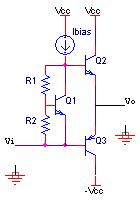
\includegraphics{schematics/classABvbemultiplier.PNG}
\end{center}
An alternate class AB output stage replaces the two diodes with a $V_{BE}$ multiplier.
From (\ref{eq:vbe_multiplier_Vo})

\begin{equation}
V_{CE1} = V_{BE1}\left(1+\frac{R_{1}}{R_{2}}\right)
\end{equation}

and

\begin{equation}
I_{\text{BIAS}} = I_{R} + I_{C1}
\end{equation}

where $I_{R}$ is the current through the resistors $R_1$ and $R_2$. $I\sub{BIAS}$ can be any current source implementation, such as a current mirror.

This biasing scheme is considerably more flexible than the two diode scheme since any bias voltage can be set using only the ratio of $R_1$ and $R_2$ and an appropriate $I\sub{BIAS}$.
%TODO: figure out the transfer function better

\subsection{Class AB output stage with input buffer transistors}
\begin{center}
	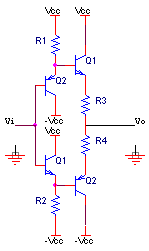
\includegraphics{schematics/classABinputbuffers.PNG}
\end{center}
In this circuit the components between the output transistors' bases is again replaced (and $R_3$ and $R_4$ have been added for temperature stability).
$Q_1$ and $Q_2$ are simply emitter followers and $R_1$ and $R_2$ determine the bias current.
If $V_{I} = V_{O} = 0$ and assuming $V_{EB1} \approx V_{BE2} \approx 0.6V$ (typical values in the forward active region), the voltage across $R_1$ and $R_2$ is $V_{CC}-V_{EB1}$ and $V_{CC}-V_{BE2}$, respectively. The desired bias currents, neglecting the small $I_{B3}$ and $I_{B4}$, are therefore

\begin{equation}
I_{E1} \approx \frac{V_{CC}-V_{EB1}}{R_{1}}
\end{equation}

\begin{equation}
I_{E2} \approx \frac{V_{CC}-V_{BE2}}{R_{2}}
\end{equation}

Since all the transistors are configured as emitter followers, the voltage gain of this output stage, like the preceding circuits, is approximately unity.
The current gain, however, is substantial.
To find the approximate current gain, note that

\begin{equation}
i_{i} = i_{b2} - i_{b1}
\end{equation}

and (neglecting the voltage drops across $R_3$ and $R_4$)

\begin{equation}
i_{b1} \approx \frac{V_{CC}-(v_{i}+v_{eb})}{(1+\beta)R_1}
\end{equation}

and

\begin{equation}
i_{b2} \approx \frac{(v_{i}-v_{be})-V_{CC}}{(1+\beta)R_2}
\end{equation}

so that

\begin{equation}
i_{i} \approx \frac{2v_{i}}{(1+\beta)R}\text{, }R = R_3 = R_4
\end{equation}

Invoking the fact that

\begin{equation}
i_{o} = \frac{v_{o}}{R_{L}} \approx \frac{v_{i}}{R_{L}}
\end{equation}

the current gain is

\textcolor{red}{
\begin{equation}
\frac{i_{o}}{i_{i}} \approx \frac{(1+\beta)R}{2R_{L}}
\end{equation}
}

$\beta_{F}$ is usually large, so the current gain (and thus the power gain) is usually significant. \autocite[598-599]{microelectronics-neaman}

\subsection{Class AB output stage with Darlington pairs}
\begin{center}
	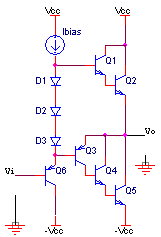
\includegraphics{schematics/classABdarlington.PNG}
\end{center}
This class AB output stage takes into account the fact that, in \ac{ic} process technologies, \textit{pnp} transistors typically have a much lower $\beta_{F}$ than \textit{npn} transistors.
Assuming individual \textit{npn} and \textit{pnp} transistors have current gains of $\beta_{n}$ and $\beta_{p}$, respectively, the composite transistor formed by $Q_1$ and $Q_2$ has an effective current gain of approximately $\beta_{n}\beta_{n}$ and the composite transistor formed by $Q_3$, $Q_4$, and $Q_5$ has an effective current gain of approximately $\beta_{p}\beta_{n}\beta_{n}$.
Since $\beta_{n} >> \beta_{p}$ the effective current gains of the composite transistors are approximately equal. \autocite[601-602]{microelectronics-neaman}

$Q_6$ is configured as an emitter follower, and the three diodes reduce the deadband by matching the three $V_{BE}$ drops from $Q_1$, $Q_2$, and $Q_3$.
Since all the transistors are configured as emitter followers, the transfer function is approximately the same as that of the simple class AB output stage.

%\section{$\mu 741$ op amp output stage (GHLM p. 381)}